\chapter{Experimental results}
\label{chapter:res}


\section{Simulating a crowd sensing campaign}
\label{sec:res-crowd}

We used our simulator in order to determine the results of multiple crowdsensing campaign located inside a city park. We used park Herastrau\footnote{\url{http://www.herastrauparc.ro/}}, in Bucharest, Romania as a case study. The geographical data, that describes the spatial mapping of the park was obtained from Open Street Maps. To be more precise the area consists of three polygons, that describe the shape of the park and the lake that spans across the park area.

To offer an idea on the difficulty of determining the number of required pedestrians to cover the entire area of the park, take the air quality campaign. It has a sensing radius of $3m$. This means that a pedestrian is able to cover approximatively $28m^2$ at a moment of time. We calculated the area of Herastrau park to be $1404409m^2$. This is consistent with the area calculated by the park managers. The result includes errors from the grid sampling method and from transformation from geographic coordinate system (GPS coordinates) to the metric system. Simply dividing the two values $1,404,409/28$ shows that we would need over $50,000$ participants. As we show later in this section, because in this solution mobility is not considered, the resulting number is far higher compared to the value obtained through simulations. 

We run our simulator using three different scenarios. These scenarios pertain to three distinct crowdsensing campaigns. For all scenarios we simulated an hour of movement. We varied the number of pedestrians from 1 to 3,000 (the results did not differ much after this value) and calculated the percentage of the covered area for each value. We chose one hour as this is an appropriate time period for which a participant would be willing to visit a park. The results for all simulations are presented in Figure \ref{fig:all}.

\begin{figure}
    \centering
    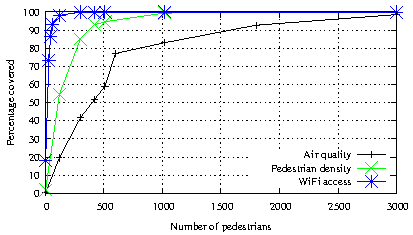
\includegraphics{src/gnuplot/all.pdf}
    \caption{Percentage of area of interest covered for different scenarios and different number of participants}
    \label{fig:all}
\end{figure}

\paragraph{Air quality - with a sensing radius of $3m$} 
This is one of the most difficult crowd sensing campaigns to implement. While the other two examples only require special software on the smartphones of regular pedestrians, this one also requires a specialized device. The smartphone still serves the purpose of communication and data processing. This has been done before~\cite{antonic2014urban} in Zagreb.

For air quality the range is the smallest, technically the sensor can only measure air that directly touches the device, however, it is safe to assume that the air in the surrounding area has the same quality, so the radius was approximated to $3m$. In order to reach a percentage of 98\% covered area, we require around 3000 persons.

\paragraph{Pedestrian density - with a sensing radius of $10m$}
In order to estimate pedestrian density, we can take advantage of the fact that smartphones are ubiquitous. All smartphones have Bluetooth modules and a lot of users simply leave them active. This module regularly sends frames that can be detected. Based on these frames we can estimate the number of pedestrian around a sensor. We estimate an appropriate sensing distance to be of $10m$, according to the Bluetooth specifications. We can see that a coverage of almost 100\% is reached at about 1000 participants.

\paragraph{WiFi access - with a sensing radius of $100m$}
In order to determine WiFi access we need to identify the number of available, open hotspots in the area. Any device with a WiFi module can receive beacon frames in order to determine what hotspots are around it and what WiFi networks it can connect to. The sensing radius, set according to the WiFi specifications, is of 100m and covers an area of $31415m^2$. We can see that approximatively 300 participants are needed to cover the area of the park in one hour.

To conclude we estimate that a successful crowd sensing campaign would require a coverage of at least 95\% of the interest area. This is not always the case as some campaigns may only require an estimate on the measured values. When the goals are as high as 95\% of the covered area, for the three case studies we proposed we obtain values for the optimal number of individuals in the order of hundreds or thousands of people. Figure \ref{fig:comparison} shows these results in more detail.

\begin{figure}
    \centering
    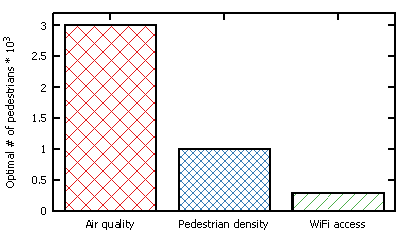
\includegraphics{src/gnuplot/comp.pdf}
    \caption{Comparison of scenarios, required number of participants in order to cover 95\% of the interest space}
    \label{fig:comparison}
\end{figure}

The number of individuals and sensing radius are not the only factors that affect the percentage of the covered area. The duration of the campaign also needs to be considered. In order to show the effect time has on a crowd sensing campaign we choose to exemplify it on the air quality scenario with 2000 participants. The results are presented in Figure \ref{fig:time}. Here, time is varied in 10 minute steps, from zero to two hours. This shows the importance of the duration of the campaign. However, the duration of a campaign cannot be easily controlled.

\begin{figure}
    \centering
    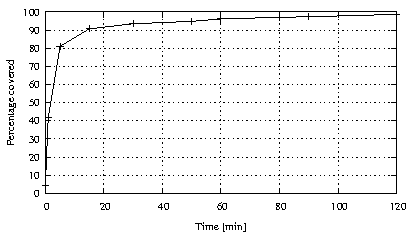
\includegraphics{src/gnuplot/time.pdf}
    \caption{Duration of campaign, Air quality, 2000 participants}
    \label{fig:time}
\end{figure}


\subsection{Discution}
\label{sec:res-crowd-discution}

In the previous section we showed how many people are required in order to have a successful crowdsensing campaign. Having this data, gives one a clear idea on what are the requirements, but it does not offer a clear view on what to expect. In order to set correct expectations, one would need to determine how many people can take part in a crowdsensing campaign. This also enables the organizers to set appropriate incentives.

The willingness of people to take part to a crowdsensing campaign is primarily influenced by the ease of access to the area of interest. People are unlikely to come from a different city just to participate in such an event. In order to determine the number of people that have access to the interest space we used a spatial interaction model.

We used an ArcGis\footnote{\url{https://www.arcgis.com/}} service in order to determine demographic information. From it, we extracted the number of people living in a specific area, in our case, the city of Bucharest. The map was split in a grid of 5 by 5 cells. The size and number of cells were chosen based on the minimum area accepted by the ArcGis service for demographics. Every cell was given an accessibility rating (A) using the model in equation \ref{eq:A}.

\begin{equation} 
A =  \frac{S_{park}^\alpha}{d_{cell-park}^\beta } 
\label{eq:A}
\end{equation}

where

\begin{itemize}
\item \( S_{park} \) - the total area of the park,
\item \(d_{cell-park}\) - Hamiltonian distance between the centroids of the cell and park,
\item \(\alpha\) - represents the effect that the dimension of the park has on the parks attractiveness,
\item \(\beta\) - describes the will of a person to travel to a destination.
\end{itemize}

We chose \(\alpha\) = 0.85 and \(\beta\) = 1.91 according to a study \cite{zhang2011modeling} that modeled the spatial accessibility to parks.

In the grid with the maximum rating, it is considered that all the people living in that area have access to the park. Further, the percentage of the total population that lives in a zone and has access to the park is calculated relatively to the maximum rating. Figure \ref{fig:access} represents the results for the accessibility rating of the cells that compose the map of Bucharest. A more detailed view is presented in \ref{chap:acc-rating}.

\begin{figure}
    \centering
    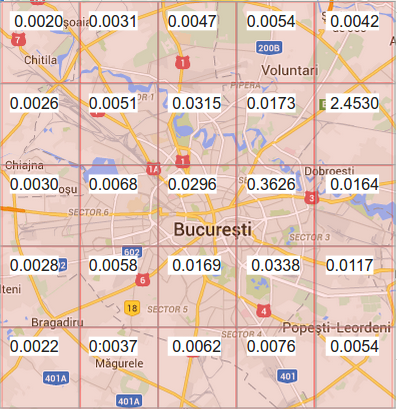
\includegraphics[width=0.5\textwidth]{src/img/Bucharest-Rating.png}
    \caption{Accessibility ratings to park Herastrau}
    \label{fig:access}
\end{figure}

Considering the area of Park Herastrau, the results suggest that the estimated maximum number of possible participants to a crowd sensing study could be around 158,312 people. By taking into account the penetration of smartphones in Romania, of 27.9\% as stated in \cite{poushter2016smartphone}, the number of possible participants is lowered to 44169.

This number is further decreased when we consider the willingness of people to partake in a crowdsensing campaign. However, the value can be used as a maximal boundary. If a crowdsensing campaign for park Herastrau requires a number of individuals larger than the 44,169 value, it is certain that the campaign will not successfully generate a complete data set. Even when incentives are used it is unlikely that they would be significant enough in order to reach this value.

In park Herastrau the scenarios we propose require different numbers of participants. These numbers represent between 1\% and 7\% (these percentages are obtained by comparing the results presented in Figure \ref{fig:comparison} to the value obtained in the previous paragraph) of the number of people that have access to the park and own a smartphone. We believe it is reasonable to assume that with proper incentives campaigns that require fewer participants can be successful (In our case the crowdsensing campaign for determining WiFi access). Campaigns that require a larger number of participants require stronger incentives.

\section{Accelerometers}
\label{sec:res-acc}

\subsection{Gestures}
The first part of implementing the use case in which we recognize gestures like walking, climbing stairs or using an elevator, is capturing real datasets with these movement, that will be used next in training the gesture recognition pipele and also when building test datasets.

This part was created using an Android application which enabled the user to record accelerometer data between two point in time. The device used for capturing data is a Nexsus 5, with InvenSense MPU-6515 as an Inertial system. The captured data is associated to one person, walking on different surfaces, using different stairs and elevators. The sampling rate is considered 2 microseconds.

The important part on this phase was to understand the nature of the gestures. In figure \ref{fig:xyz-stairs-up} an example of recorded data when going up a stair is displayed. We can se that most of the movement happens vertically, so we consider only recognising gestures based on the vertical axis. Other captured data can be seen in \ref{fig:xyz-stairs-down}, for going down a stair, \ref{fig:xyz-walking} for one step in the process of walking.

One problem for this phase is to segment correctly the captured data, so that the training is correct. For this the Android application enables the user to delimit one step in the proccess of moving, but using only user input is not enought, as it is not very precise. This means that additional manual work is needed so that the training data is correctly segmented.

Another problem is the orientation of the phone, when the data is captured. For this the training and testing datasets include different position like in hand or in the pocket.

The results show that taking a step in the process of walking is simillar with a step when climbimg a stair. The difference sits in the initaial part of the step, when the leg getts up, as in stairs this action has a greater amplitude and also has a larger duration. Also, when the leg touches, when on stairs the acceleration is larger on the stairs.

When comparing going up or down a stair way, we can see that the movement are quite opposite and that going up taks more acceleration that going down.

In terms of elevator movement, the accelerations involved have the tendacy to jump from a positive value to a negative one fast.

\begin{figure}
    \centering
    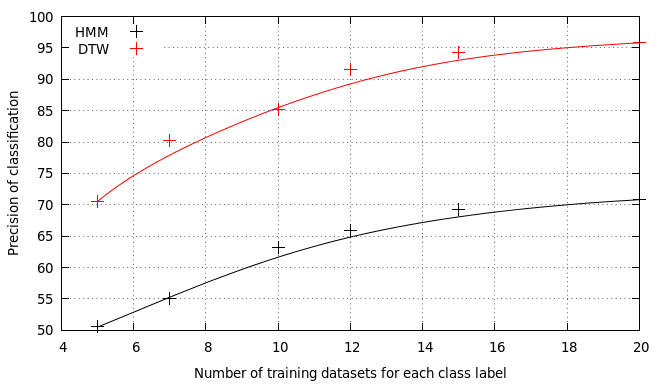
\includegraphics[width=0.7\textwidth]{src/img/comp-HMM-DTW.png}
    \caption{Accelerometer data for elevator stopping}
    \label{fig:comp-HMM-DTW}
\end{figure}


\subsection{Recognition performace}
The porpose of recognising the seven action proposed in the current use case falls to the role of the gesture recognition pipeline.

The pipeline is trained using the datasets obtained in the data aquizition phase from the Android to create the training and testing datasets.

The recognition pipeline for implementing the proposed use case included two version. The first used Hidden Markow Model and the second used Dynamic Time Warping. This algorithms were choosen because of their popularity when dealing with temporal gesture recognition.

The Hidden Markov Model additionaly needs an algorithm for future extraction, which can covert from an N-dimensional input to a one dimennsional input. For this K-Means Quantizer was used.
